\subsection{Presentation Layer}
\gls{AS}ets grafiske brugerflade består af et hovedvindue, samt en række dialog-vinduer, som bruges når produkter og kategorier skal oprettes, redigeres eller slettes. Alle vinduer er lavet ud fra et fælles designgrundlag, så alle vinduerne ligner hinanden så meget som muligt i forhold til elementerne i brugerfladen såsom knappernes placering. En skitse af, hvordan \gls{GUI} til Administrationssystemet ser ud kan ses på figur \ref{fig:admin_design}.

\begin{figure}[H]
	\centering
	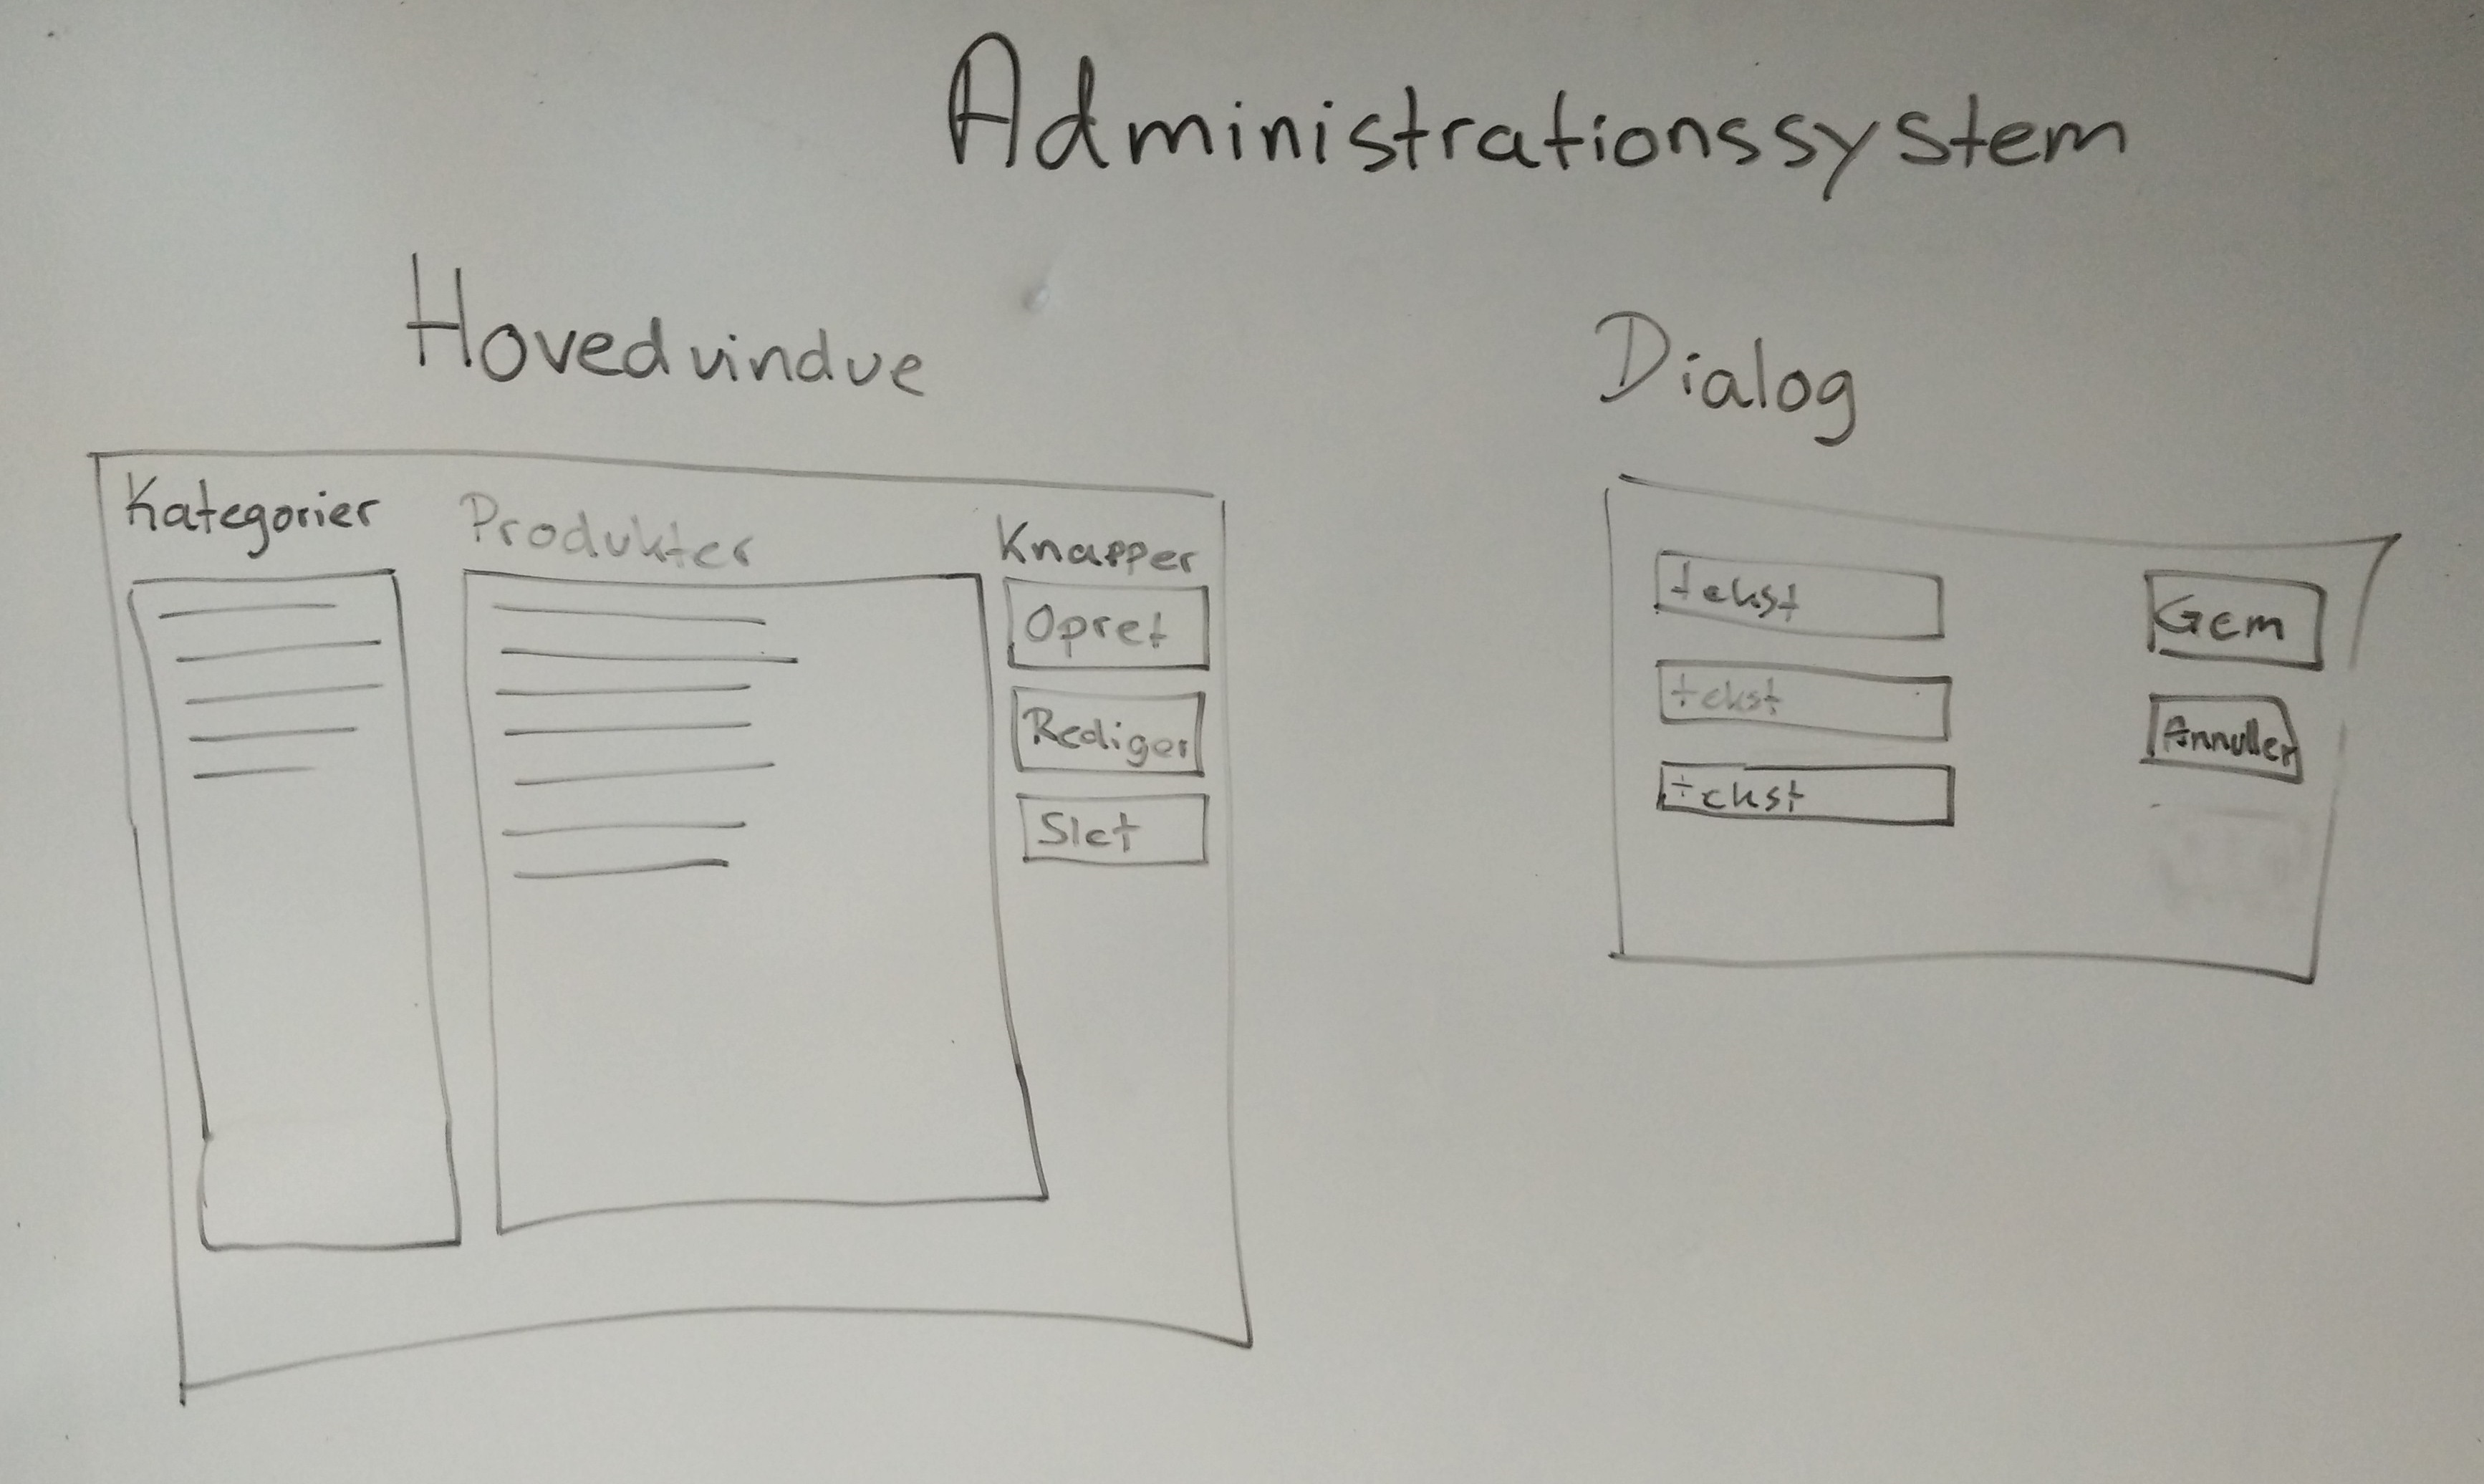
\includegraphics[width=1\textwidth]{Systemdesign/backend/Images/AdminDesign}
	\caption{Skitse af design til \gls{AS}}
	\label{fig:admin_design}
\end{figure}

Der er to dele: hovedvindue og dialog. Hovedvinduet er det første vindue der vises når programmet starter, og hvor alle andre vinduer åbnes fra, vha. knapper. Hovedvinduet har tre dele: en liste af produktkategorier, en liste af produkter i den valgte produktkategori, samt en række knapper til at administrere systemet.

Dialogdesignet er et generisk design for de dialogvinduer der åbnes, når \gls{SB} ønsker at udføre en handling, som f.eks. at oprette et produkt. Dialogdesignet er lavet, så det ligner hovedvinduet så meget som muligt. Knappernes placering er ens i hovedvinduet og dialogvinduerne. I dialogdesignet er der på skitsen (figur \ref{fig:admin_design}) tre bokse med "tekst" i. Disse viser hvor eventuelle tekstbokse til input skal placeres. Disse tekstbokse kan udskiftes med lister, tekst eller andet der er relevant for vinduet.\\

Det endelige design af \gls{AS} kan ses nedenfor, på figur \ref{fig:admin_final_dialog} og \ref{fig:admin_final_dialog}.

\begin{figure}[H]
	\centering
	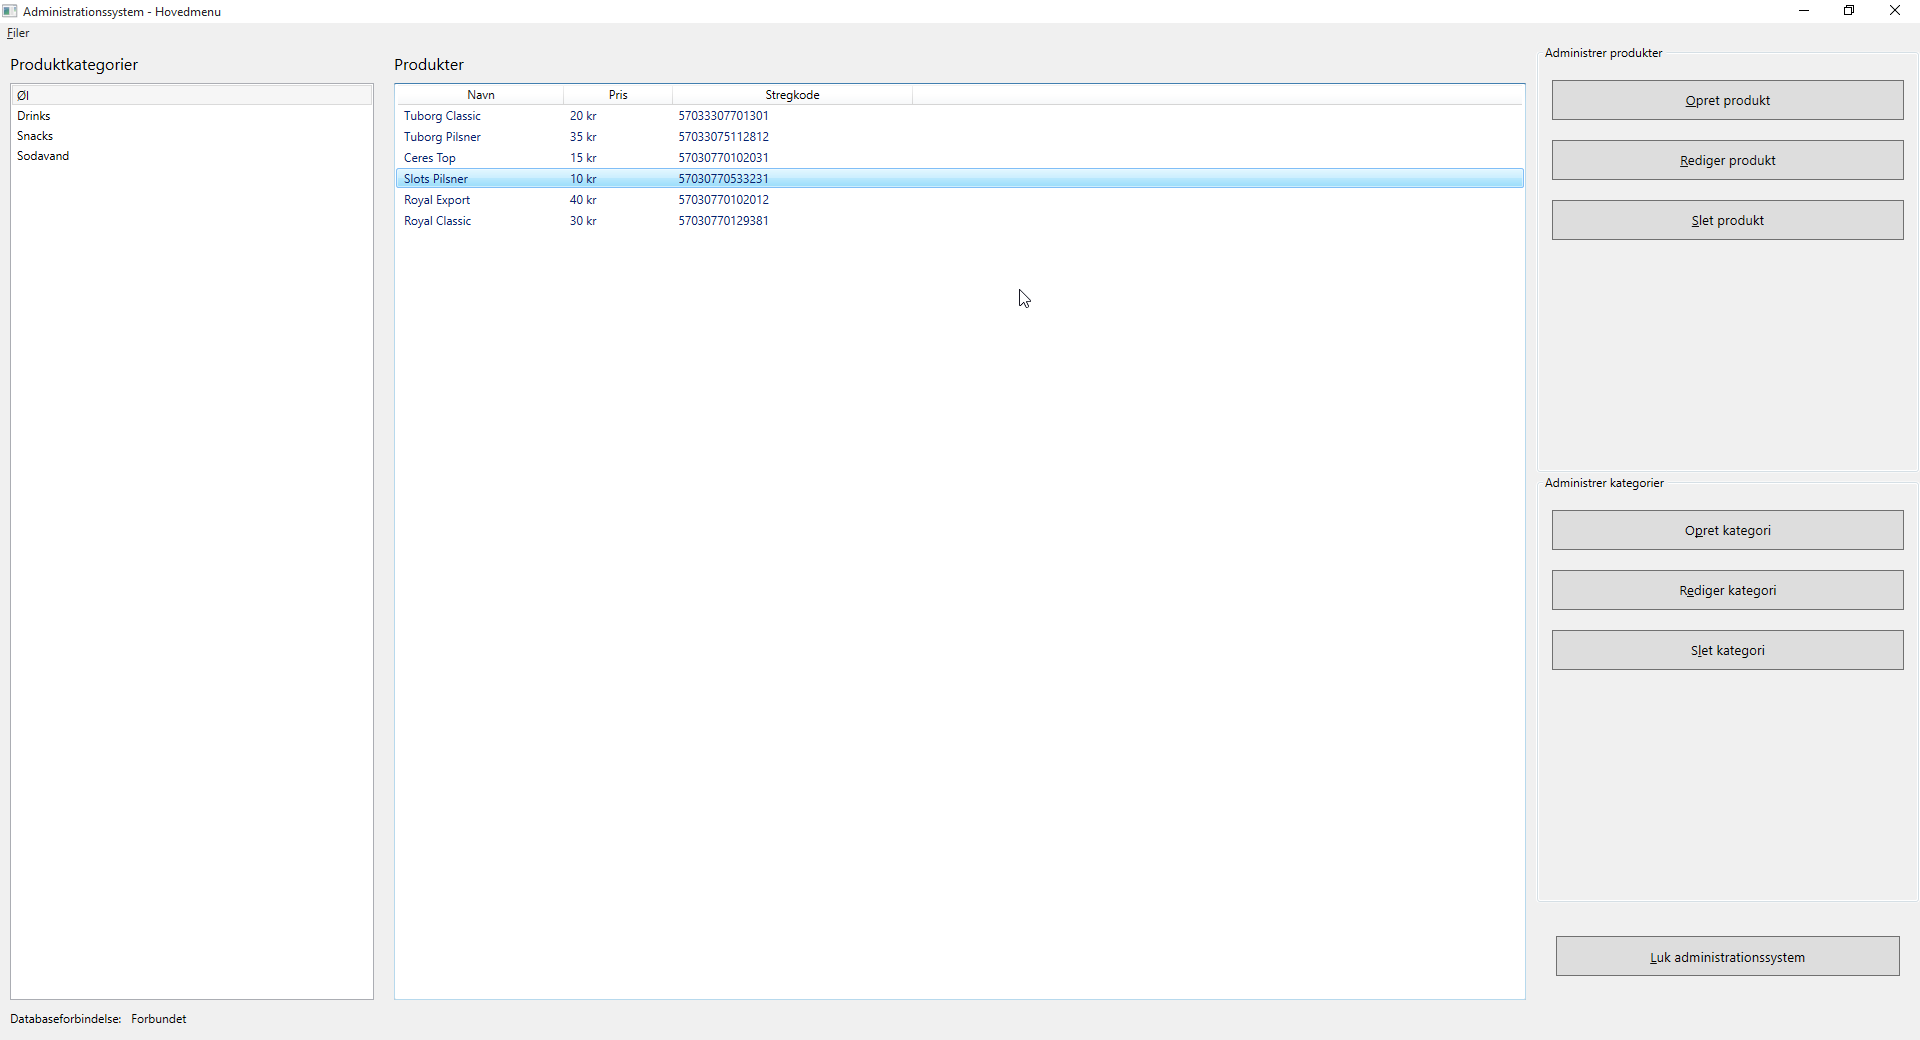
\includegraphics[width=1\textwidth]{Systemdesign/backend/Images/AdminDesignHovedvindue}
	\caption{Det endelige udseende af \gls{AS} - Hovedvindue}
	\label{fig:admin_final_hovedvindue}
\end{figure}

\begin{figure}[H]
	\centering
	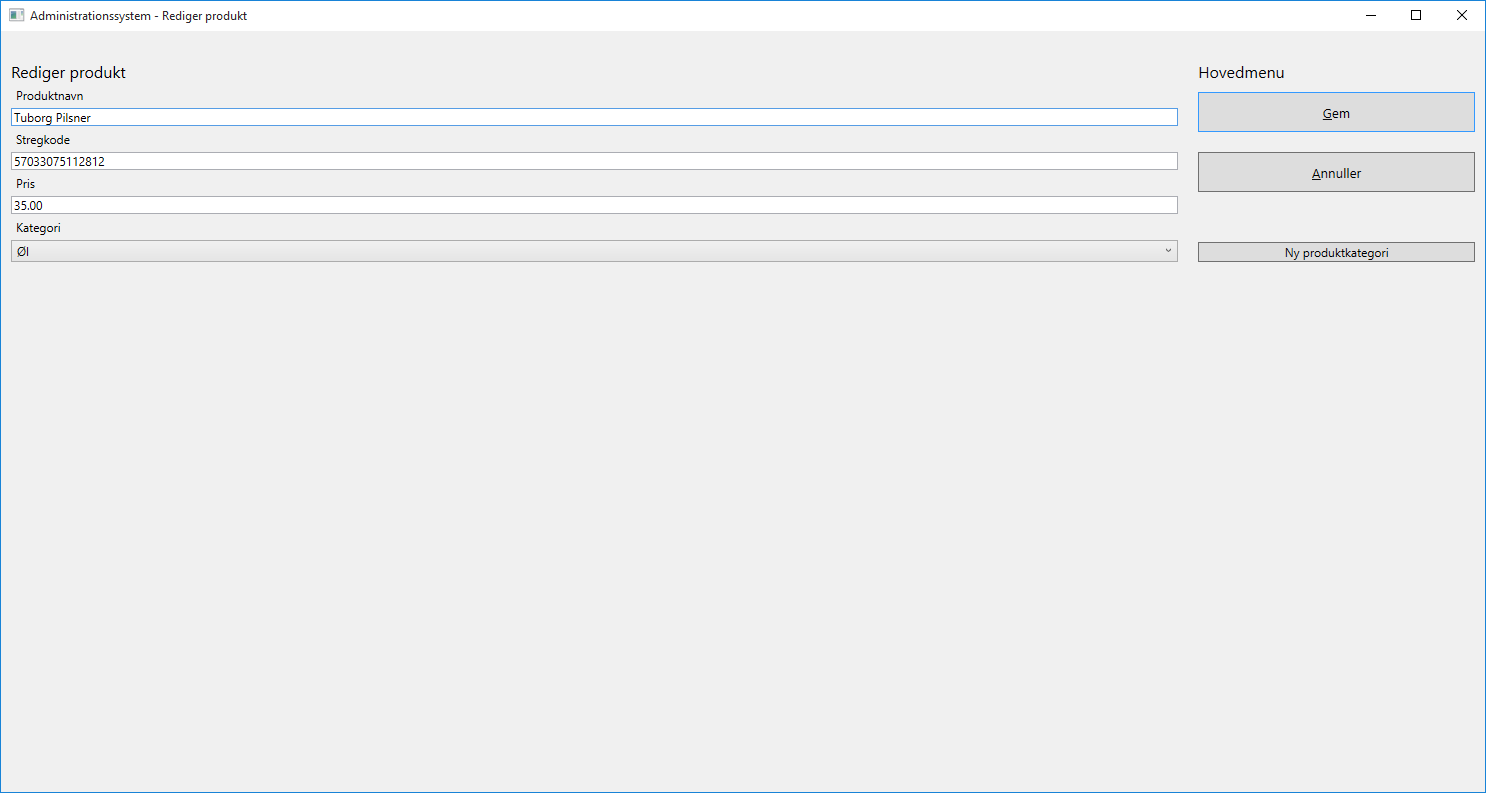
\includegraphics[width=1\textwidth]{Systemdesign/backend/Images/AdminDesignRedigerProdukt}
	\caption{Det endelige udseende af \gls{AS} - Dialogvindue (Rediger produkt)}
	\label{fig:admin_final_dialog}
\end{figure}

Som det ses på figur \ref{fig:admin_final_hovedvindue} er designet meget lig det skitserede (figur \ref{fig:admin_design}). Kategorilisten er i venstre side, produkter i kategorien vises i midten og til højre er diverse knapper. Der er to sæt af knapper, tre til at oprette, slette og redigere produkter og tre til at oprette, slette og redigere kategorier.\\

I dialogvinduet (figur \ref{fig:admin_final_dialog}) er der tre tekstbokse, en liste over kategorier og tre knapper. Alle dialogvinduer følger dette design og afviger kun fra hinanden ved antallet af tekstbokse og knapper. Positionerne forbliver altid de samme.

Den eneste dialog, der afviger en del fra designet er til "Slet produkt". Dette er blot et popup-vindue med Ja/Nej-mulighed. Et billede af popup-vinduet kan ses på figur \ref{fig:admin_final_sletprodukt}.

\begin{figure}[H]
	\centering
	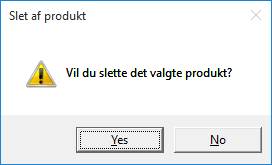
\includegraphics[width=0.4\textwidth]{Systemdesign/backend/Images/AdminDesignSletProdukt}
	\caption{Det endelige udseende af \gls{AS} - Dialogvindue for Slet produkt}
	\label{fig:admin_final_sletprodukt}
\end{figure}

Popup-vinduet på figur \ref{fig:admin_final_sletprodukt} er implementeret i MainWindowViewModel, da funktionaliteten af vinduet syntes for simpelt til at kunne retfærdiggøre at skulle lave et helt dialogvindue med tilhørende ViewModel.\\\\
Foruden dette, er der benyttet settings til at sætte IP og port til \gls{CS}, således disse bliver gemt. Disse indstillinger kan ændres ved at trykke på Filer og derefter Indstillinger. Før man gemmer port og IP, kan man teste forbindelsen.